%\bibliographystyle{wdg_jmc}
\bibliographystyle{plain}
\documentclass[10pt]{amsart}

%\usepackage{../../sasha_ams}
%\usepackage{makeidx}
%\usepackage{sasha_ams}
\usepackage{hyperref}
\usepackage{srcltx}
\usepackage{xcolor}
\usepackage{graphicx}

%\usepackage{pst-plot}
%\usepackage{pst-text}
%\usepackage{pst-eucl,pstricks-add}


\newcommand{\an}{\noindent\color{blue} Andrey: }{}

\newtheorem{theorem}{Theorem}[section]
\newtheorem{lemma}[theorem]{Lemma}
\theoremstyle{definition}
\newtheorem{example}[theorem]{Example}
\newtheorem{problem}[theorem]{Problem}
\newtheorem{remark}[theorem]{Remark}
\newtheorem{definition}[theorem]{Definition}
\newtheorem{proposition}[theorem]{Proposition}
\newtheorem{corollary}[theorem]{Corollary}


\DeclareMathOperator{\RST}{{\bf ST}}
\DeclareMathOperator{\Mat}{{Mat}}
\DeclareMathOperator{\size}{{size}}
\def\P{{\mathbf{P}}}
\def\e{{\mathbf{e}}}
\def\NP{{\mathbf{NP}}}
\def\WP{{\mathbf{WP}}}
\def\SSP{{\mathbf{SSP}}}
\def\ZOE{{\mathbf{ZOE}}}
\def\BMP{{\mathbf{BMP}}}
\def\SMP{{\mathbf{SMP}}}
\def\BSMP{{\mathbf{BSMP}}}
\def\BKP{{\mathbf{BKP}}}
\def\KP{{\mathbf{KP}}}
\def\IKP{{\mathbf{IKP}}}
\def\BIKP{{\mathbf{BKP}}}
\def\GWP{{\mathbf{GWP}}}
\def\SP{{\mathbf{MP}}}
\def\iden{{\mathbf{1}}}
\def\KOP{{\mathbf{KOP}}}
\def\SSOP{{\mathbf{SSOP}}}
\def\SMOP{{\mathbf{SMOP}}}
\def\BSMOP{{\mathbf{BSMOP}}}
\def\BGWP{{\mathbf{BGWP}}}
\def\AGP{{\mathbf{AGP}}}
\def\dumb{simple} %short? basic? tame?
\def\nondumb{non-simple} %long? essential?

\title{Knapsack problems in free products of groups}

\author[]{Elizaveta Frenkel, Andrey Nikolaev, and Alexander Ushakov}

\address{Elizaveta Frenkel, Moscow State University, GSP-1, Leninskie gory, 119991,
Moscow, Russia}
\email{lizzy.frenkel@gmail.com}

\address{Andrey Nikolaev, Stevens Institute of Technology, Hoboken, NJ, 07030 USA}
\email{anikolae@stevens.edu}

\address{Alexander Ushakov, Stevens Institute of Technology, Hoboken, NJ, 07030 USA}
\email{aushakov@stevens.edu}



\thanks{The work of the third author was partially supported by NSF grant DMS-0914773.}



\begin{document}
\begin{abstract}
We study complexity of knapsack and related problem in free products of groups.

\noindent
{\bf Keywords.} Subset sum problem,  knapsack problem, bounded subgroup membership problem, free products, hyperbolic groups, nilpotent groups.

\noindent
{\bf 2010 Mathematics Subject Classification.} 03D15, 20F65, 20F10.
\end{abstract}
\maketitle


\tableofcontents

\section{Introduction}\label{sec:intro}


\subsection{Motivation}\label{sub:motivation}
In this paper, following~\cite{MNU1}  we continue the research on  non-commutative discrete (combinatorial) optimization. Specifically, we set out to study the properties of the subset sum problem in free products of groups. It turns out that so-called knapsack-type problems such as the aforementioned subset sum problem, the knapsack problem, and the bounded submonoid membership problem share a certain common ground that allows to approach these problems in a unified fashion. Thus our research both presents certain known facts about these algorithmic problems in a new light, and widens the class of groups with known complexity of the knapsack-type problems.

We refer to~\cite{MNU1,MNU2} for the initial motivation for the study of non-commutative discrete optimization, the set-up of the problems, and initial facts on non-commutative discrete optimization.

\subsection{Results and open questions}\label{sub:results}
As we said in the preceding section, we investigate properties of the subset problem in groups ($\SSP$). In the context of our study, it is natural to view this problem, along with the bounded knapsack problem ($\BKP$) and the bounded submonoid membership problem ($\BSMP$) (see Section~\ref{sec:problems} for definitions), as special cases of a more general discrete optimization problem formulated in terms of graphs labeled by group elements, which we termed the {\em acyclic graph problem} ($\AGP$).

We establish connection between $\SSP$, $\BKP$, $\BSMP$ and $\AGP$. We show that $\AGP$ is $\P$-time solvable in all known groups where $\SSP$ is. Further, we show that free products preserve polynomial time $\AGP$, i.e. $\AGP(G* H)\in\P$ if and only if $\AGP(G)\in\P$ and $\AGP(H)\in\P$. As a consequence, we obtain that $\SSP$, $\BKP$, $\BSMP$ are polynomial time solvable in a wide class of groups. We also observe that the same is false for direct products, i.e. that $\AGP(G)\in\P$, $\AGP(H)\in\P$ does not imply $\AGP(G\times H)\in\P$ (unless $\P=\NP$). Finally, we observe that $\KP$ in a free product $\P$-time reduces to $\BKP$.

It remains an open question whether there is a group with polynomial time $\SSP$ but $\AGP$ is $\NP$-hard.

\section{Preliminaries}\label{sec:prelim}\label{sec:problems}

In this paper we follow terminology and notation introduced in \cite{MNU1}. 
For convenience, below we formulate the algorithmic problems mentioned in Section~\ref{sec:intro}. We collectively refer to these problems as {\it knapsack-type} problems in groups.

Elements in $G$ generated by a finite or countable set $X$ are given as words over the alphabet  $X \cup X^{-1}$.

\medskip
\noindent{\bf The subset sum  problem $\SSP(G,X)$\index{$\SSP(G,X)$}:}
Given $g_1,\ldots,g_k,g\in G$ decide if
  \begin{equation} \label{eq:SSP-def}
  g = g_1^{\varepsilon_1} \ldots g_k^{\varepsilon_k}
  \end{equation}
for some $\varepsilon_1,\ldots,\varepsilon_k \in \{0,1\}$.

%\begin{remark}
%As we show in~Subsection~\ref{sec:general-properties} (Lemma~\ref{le:SSP_reduction}), if $X$ and $Y$ are two {\em finite} generating sets for a group $G$, $\SSP(G,X)$ is in $\P$ if and only if $\SSP(G,Y)$ is in $\P$. However, if at least one of the sets $X$ and $Y$ is infinite, the same is false in general (see Example~\ref{ex:inf_gen_set}).
%With that in mind, we often write $\SSP(G)$ if a finite generating set is implied, or if the generating set is fixed explicitly. We also often write $\SSP$ instead of $\SSP(G)$ when we talk about the problem in general, or when the group $G$ is clear from the context. The same applies to all problems we introduce here and in Section~\ref{se:formulation}.
%\end{remark}

\medskip
\noindent
{\bf The knapsack problem $\KP(G,X)$\index{$\KP(G,X)$}:}  Given $g_1,\ldots,g_k,g\in G$
decide if
\begin{equation}\label{eq:IKP-def}
g =_G g_1^{\varepsilon_1} \ldots g_k^{\varepsilon_k}
\end{equation}
for some  non-negative integers $\varepsilon_1,\ldots,\varepsilon_k$.


\medskip

%There is also a variation of this problem, termed {\it integer knapsack problem} ($\IKP$), when the coefficients  $\varepsilon_i$ are arbitrary integers. However, it is easy to see that $\IKP$ is $\P$-ible to $\KP$ for any group $G$ (see Section   \ref{sec:general_properties}).

The third problem is equivalent to $\KP$ in the classical (abelian) case, but in general it is a completely different problem that is of prime  interest in algebra:

\medskip
\noindent
{\bf Submonoid membership problem $\mathbf{SMP}(G,X)$\index{$\SMP(G,X)$}}:  Given elements $g_1,\ldots,g_k,g\in G$
decide if $g$ belongs to the submonoid generated by $g_1, \ldots, g_k$ in $G$, i.e., if the following equality holds for some $g_{i_1}, \ldots, g_{i_s} \in \{g_1, \ldots, g_k\}, s \in \mathbb{N}$:
\begin{equation}\label{eq:SMP-def}
g = g_{i_1}, \ldots, g_{i_s}.
\end{equation}

\medskip
The restriction of $\SMP$ to the case when the set of generators $\{g_1, \ldots,g_n\}$ is closed under inversion (so the submonoid is actually a subgroup of $G$) is  a well-known problem in group theory, called the {\em generalized word problem} ($\GWP$) or the {\em uniform subgroup membership problem} in $G$.
%There is a huge bibliography on this subject, we mention some related results  in Section \ref{sec:results}.

As usual in complexity theory, it makes sense to consider the {\em bounded} versions of $\KP$ and $\SMP$, at least they are always decidable in groups where the word problem is decidable. In this case the problem is to verify  if the corresponding equalities (\ref{eq:IKP-def}) and  (\ref{eq:SMP-def}) hold for a given $g$ provided that the number of factors in these equalities  is bounded by a natural number $m$ which is given in the unary form, i.e., as the word $1^m$. In particular, the bounded knapsack problem ($\BKP$) for a group $G$ asks to decide, when  given $g_1,\ldots,g_k,g\in G$ and $1^m\in\mathbb N$, if the equality (\ref{eq:IKP-def}) holds for some
$\varepsilon_i \in \{0,1, \ldots, m \}$.
This problem  is  $\P$-time equivalent to  $\SSP$ in $G$ (see the definition of $\P$-time reduction below), so it suffices for our purposes to consider only $\SSP$ in groups.
On the other hand,  the bounded $\SMP$ in $G$ is very interesting in its own right.


\medskip \noindent
{\bf Bounded submonoid membership problem $\BSMP(G,X)$\index{$\BSMP(G,X)$}:}
Given $g_1, \ldots g_k, g \in G$ and $1^m \in \mathbb{N}$ (in unary)
decide if $g$ is equal in $G$ to a product of the form
$g=g_{i_1}\cdots g_{i_s}$, where $g_{i_1}, \ldots, g_{i_s} \in \{g_1, \ldots, g_k\}$ and  $s\le m$.


%\medskip
%We mention in passing that there are also {\it search} and {\it optimization} variations of these problems which we are not going to touch on within this paper.

%There are also  interesting and important {\it search} variations of the decision problems above, when the task is to find an actual solution to equations (\ref{eq:SSP-def}), (\ref{eq:IKP-def}), or (\ref{eq:SMP-def}), provided that some solution  exists (see Section \ref{sec:general_properties} for more details on this). In most cases we solve both the decision and search variations of the problems above simultaneously, while establishing the time complexity upper bounds for the algorithms.  However, as in the classical case, perhaps the most interesting variations  of the search problems are their {\it optimization} versions. It seems these problems were never formally stated before for groups, so we discuss them in a bit more detail here, leaving a more thorough discussion for Section \ref{sec:general_properties}.

\medskip
Recall that a decision problem $(I_1,D_1)$ is  {\em $\P$-time  reducible}
to  a problem $(I_2,D_2)$ if there is a $\P$-time computable function
$f:I_1  \to I_2$  such that for any $u \in I_1$ one has $u \in D_1 \Longleftrightarrow f(u) \in D_2$.
Such reductions are usually called either {\em many-to-one} $\P$-time reductions or Karp reductions.
Since we do not use any other reductions we omit ``many-to-one'' from the name and call them $\P$-time reductions. We say that two problem are $\P$-time equivalent if each of them $\P$-time reduces to the other.

It is not hard to see that for a problem $\Pi\in \{\SSP, \KP, \BKP, \SMP, \BSMP\}$, $\Pi(G,X_1)$ is $\P$-time equivalent to $\Pi(G,X_2)$ for any finite generating sets $X_1,X_2$, i.e. the time complexity of $\Pi(G)$ does not depend on the choice of a finite generating set of a given group $G$.
For further information concerning knapsack-type problems and their variations in groups, details regarding their algorithmic set-up, and the corresponding basic facts the reader is referred to~\cite{MNU1}.


%\medskip
%\noindent
%{\bf The subset-sum optimization problem $\SSOP(G,X)$\index{$\SSOP(G,X)$}:}  Given an instance $g_1$, $\ldots$, $g_k$, $g\in G$ of  $\SSP(G)$ find a solution, if it exists,
%$\varepsilon_1,\ldots,\varepsilon_k \in \{0,1\}$  subject to the optimization  condition that
%the sum $\sum_i \varepsilon_i$ is minimal. Otherwise, output $No \ solutions$.
%
%\medskip
%\noindent
%{\bf The knapsack optimization problem  $\KOP(G,X)$\index{$\KOP(G,X)$}:} solve the equation (\ref{eq:IKP-def}) 
%with the minimum possible number of factors.
%
%\medskip
%In fact, in Section \ref{sec:general_properties} we also discuss other variations of $\KOP$ in groups,  which are even more direct generalization of the classical $\KOP$. In this case  when given $g_1,\ldots,g_k,g\in G$ one has to find $\varepsilon_1,\ldots,\varepsilon_k \in \mathbb{N}$ for which  the product $g_1^{\varepsilon_1}\ldots g_k^{\varepsilon_k}$ is as close to $g$ (in the metric of the Cayley graph of $G$) as possible.
%
%
%\medskip
%\noindent
%{\bf The submonoid membership optimization problem $\SMOP(G,X)$\index{$\SMOP(G,X)$}:} %Let $c:G \rightarrow \mathbb N$ be a fixed function.
%Given $g_1,\ldots,g_k,g\in G$, % and $c(g_1),\ldots,c(g_k)$, 
%express (if possible) $g$ as a product
%\begin{equation}\label{eq:MSP_G}
%g =_G g_{i_1} \ldots g_{i_m}
%\end{equation}
%with the  minimum number of factors $m$.
%
%\medskip
%The submonoid membership optimization problem plays an important part in geometric group theory.  Indeed, in geometric language it asks to find a geodesic of a given element in a group (relative to a fixed finite generating set) or the distortion of a given element in a given finitely generated subgroup --- both are crucial geometric tasks.
%
%Sometimes (like in hyperbolic groups) the time complexity of the search $\SMP$ is not bounded from above by any computable function, in this case it makes sense to consider the optimization  version of the bounded $\SMP$, called $\BSMOP$, in which one has to solve $\BSMP(G)$ with the minimal possible number of factors.
%
%The formal description  of the problems above depends on the given finite (or sometimes countable) generating set $X$ of the group $G$.
%To this end if $\Pi$ is any of the algorithmic problems above then by $\Pi(G,X)$ we denote this problem for the group $G$ relative to the generating set $X$.  It
%is not hard to show (see Section \ref{sec:general_properties}) that for a given such $\Pi$, provided it is not an optimization problem, replacing one  finite
%set of generators of $G$ by another  one ends up in a problem that is $\P$-time reducible
%to the initial one.
%Therefore, the time complexity of such  problems does not depend on a finite generating set,
%it is an invariant of the group $G$.
%In view of this, we omit $X$ from the notation   and denote such problems  by $\Pi(G)$.
%
%The typical groups we are interested in here are free,  hyperbolic, abelian, nilpotent, or metabelian.  In all these groups, and this is important, the word problem is decidable in $\P$-time. We might also be interested in constructing some exotic examples of groups where the problems mentioned above have unexpected complexity.

%\subsection{Algorithmic set-up}\label{sub:setup}
%Since the knapsack-type problems were not previously studied in non-commutative setting
%it is worthwhile to say a few words on how we present the data,
%models of computations, size functions,  etc.
%(we refer to the book \cite{MSU_book:2011} for more details).
%Our model of computation is RAM (random access machines).
%
%To make the statements of the problems (from Section \ref{sec:problems})
%a bit more precise consider the following. If a  generating set $X = \{x_1,\ldots,x_n\}$ of a
%group $G$  is finite, then the {\em size}
%of the word $g = x_1\ldots x_k$ is its length $|g|=k$ and the size of
%the tuple $g_1, \ldots, g_k, g$ from $G$
%is the total sum of the lengths $|g_1| + \ldots +|g_k| +|g|$.
%
%
%If the generating set $X$ of  $G$ is infinite,
%then the size of a letter $x \in X$ is not necessarily equal to $1$,
%it depends on how we represent elements of $X$.
%In what follows we always assume that there is an efficient injective function $\nu: X \to \{0,1\}^*$ which encodes the elements in $X$
%such that for every $u \in \{0,1\}^*$ one can algorithmically recognize if $u \in \nu(X)$, or not.
%In this case for $x\in X$ define:
%    $$\size(x) = |\nu(x)|$$
%and for a word $w  = x_1 \ldots x_n$ with $x_i\in X$ define:
%    $$\size(w) = \size(x_1) + \ldots + \size(x_n).$$
%Similar to the above the size of a tuple $(g_1, \ldots, g_k, g)$ is:
%    $$\size(g_1, \ldots, g_k, g) = \size(g_1) + \ldots + \size(g_k) +\size(g).$$
%One can go a bit further and identify elements $x \in X$ with their images $\nu(x) \in \{0,1\}^*$,
%and words $w  = x_1 \ldots x_n \in X^*$ with the words $\nu(x_1) \ldots \nu(x_n) \in \{0,1\}^*$.
%This gives a homomorphism of monoids $\nu^*: X^* \to \{0,1\}^*$.
%If in addition $\nu$ is such that for any $x,y \in X$
%the word $\nu(x)$ is not a prefix of $\nu(y)$ (this is easy to arrange),
%then:
%\begin{itemize}
%    \item
%$\nu^*$ is injective,
%    \item
%$\nu^*(X^*)$ and $\nu^*(X)$ are algorithmically recognizable in $\{0,1\}^*$,
%    \item
%and for every word $v \in \nu^*(X^*)$ one can find the word $w \in X^*$ such that $\nu^*(w) = v$.
%\end{itemize}
%From now on we always assume that a generating set comes equipped with a function~$\nu$, termed {\it encoding},  satisfying
%all the properties mentioned above.
%In fact, almost  always all our generating sets $X$ are finite, and in those rare occasions when $X$ is infinite we describe $\nu$ precisely.
%
%In general, we view decision problems as pairs $(I,D)$, where $I$ is the space of instances of
%the problem equipped with a  size function $\size: I \to \mathbb N$ and
%a set $D \subseteq I$ of affirmative (positive) instances of the problem.
%Of course, the set $I$ should be constructible and size function  should be computable.
%In all our examples the set $I$ consists either of tuples of words $(g_1, \ldots,g_k,g)$ in
%the   alphabet $\Sigma_X$ for some (perhaps, infinite) set of generators $X$ of a group $G$, or,
%in the case of  $\BKP$  or $\BSMP$,
%tuples of the type  $(g_1, \ldots,g_k,g,1^m)$ where $1^m$ is
%a natural number $m$ given in unary.
%The problem $(I,D)$ is decidable if there is an algorithm ${\mathcal A}$
%that for any $x \in I$ decides whether  $x$ is in $D$ or not (${\mathcal A}$  answers ``Yes'' or ``No'').
%The problem is in class $\P$ if there is a decision algorithm ${\mathcal A}$
%with polynomial  time function with respect to the size of the instances in $I$, i.e.,
%there is a polynomial $p(n)$ such that for any $x \in I$ the algorithm ${\mathcal A}$ starts on $x$,
%halts in at most $p(\size(x))$ steps, and gives a correct answer ``Yes'' or ``No''.
%Similarly, we define problems in linear  or quadratic time, and non-deterministic polynomial time $\NP$.
%
%
%Recall that a decision problem $(I_1,D_1)$ is  {\em $\P$-time  reducible}
%to  a problem $(I_2,D_2)$ if there is a $\P$-time computable function
%$f:I_1  \to I_2$  such that for any $u \in I_1$ one has $u \in D_1 \Longleftrightarrow f(u) \in D_2$.
%Such reductions are usually called either {\em many-to-one} $\P$-time reductions or Karp reductions.
%Since we do not use any other reductions we omit ``many-to-one'' from the name and call them $\P$-time reductions.  Similarly, one can introduce linear or quadratic time reductions, etc. We say that two problem are $\P$-time equivalent if each of them $\P$-time reduces to the other.
%
%%One can similarly define $\P$-time reduction for optimization problems
%Now we define an optimization problem as a  tuple $(I,J, F,\mu,{\mathop{\mathrm{extr}}})$, where $I$ is the set of instances, $J$ is a set of solutions, $F:I \to P(J)$ is a function that for each instance $u \in I$ associate a subset  $F(u)\subseteq J$  of all feasible solutions for an instance $u$, $\mu(u,v)$ is a non-negative real function  which for $u \in I, v \in F(u)$ measures the cost of solution $v$ for an instance $u$,  ${\mathop{\mathrm{extr}}}$ is either $\min$ or $\max$. This optimization problem, given $u\in I$, asks to find $v\in F(u)$ such that $\mu(u,v)={\mathop{\mathrm{extr}}}\{\mu(u,v')\mid v'\in F(u)\}$. Given two optimization problems $P_i=(I_i,J_i, F_i,\mu_i,{\mathop{\mathrm{extr}}}_i)$, $i=1,2$, we say that $P_1$ is {\em $\P$-time reducible} to $P_2$ if there is a $\P$-time computable functions $f:I_1\to I_2$, $f_u:F_1(u)\to F_2(f(u)), u\in I_1,$ such that $v\in F_1(u)\iff f_u(v)\in F_2(f(u))$ and $\mu_1(u,v)={\mathop{\mathrm{extr}}}_1\{\mu_1(u,v')\mid v'\in F_1(u)\} \Longleftrightarrow \mu_2(f(u),f_u(v))={\mathop{\mathrm{extr}}}_2\{\mu_2(f(u),v')\mid v'\in F_2(f(u))\}$. In our consequent considerations, the functions $f_u$ are apparent from the set up and we do not mention them in our arguments. We say that two optimization problem are $\P$-time equivalent if each of them $\P$-time reduces to the other.


%\subsection{More on the formulation of the problems}
%\label{se:formulation}
%In this section we continue the discussion from the introduction on  different variations of the problems $\SSP$, $\KP$, $\SMP$ in groups.
%
%There are two ways to state search variations of the problems: the first one, as described  in the introduction, considers only feasible instances of the problem, i.e.
%% those instances of the problem which are in the ``yes'' part of the problem,
%we assume that a solution to the instance exists; the second one is stronger, in this case it is required to solve the decision problem and simultaneously find a solution (if it exists) for a given instance. The former requires only a partial algorithm, while the latter asks for a total one. The weaker version of the problems $\SSP(G)$, $\KP(G)$, $\SMP(G)$ is always decidable in groups $G$  with decidable word problem, while the stronger one might be undecidable (for instance, $\SMP$ in hyperbolic groups). In this paper we consider the stronger version of the search problems.
%
%We mentioned in the introduction that the knapsack optimization problem ($\KOP$) may have different formulations in the non-commutative groups.
%Now we explain what we meant.
%
% Recall first, that perhaps the most typical version of the classical $\KOP$ asks, when given positive integers $a_1, \ldots, a_k,a$ to find $\varepsilon_1, \ldots, \varepsilon_k \in \mathbb{N}$ such that the sum  $ \varepsilon_1a_1 + \ldots +  \varepsilon_ka_k$ is less or equal to $a$ but  maximal possible under this restriction.  One can  generalize this  to  non-commutative groups as follows.
%
% \medskip \noindent
% {\bf $\KOP1(G,X)$\index{$\KOP1(G,X)$}:} Given $g_1,\ldots,g_k,g\in G$
%find $\varepsilon_1, \ldots, \varepsilon_k \in \mathbb{N}\cup\{0\}$ with the least
%possible distance between $g$ and $g_1^{\varepsilon_1} \ldots g_k^{\varepsilon_k}$ in the Cayley graph $Cay(G,X)$. 
%
%\medskip
% This formulation allows solutions with the ``total weight'' higher than the capacity of the knapsack. To define precisely when a given solution fits in geometrically  in the knapsack we need the following. For elements  $g, h, u \in G$  we say that $u$  {\it belongs to the segment $[g,h]$} if there is a geodesic path in $Cay(G,X)$ from $g$ to $h$ that contains $u$.   Now we can formulate the problem.
%
%  \medskip \noindent
% {\bf $\KOP2(G,X)$\index{$\KOP2(G,X)$}:} Given $g_1,\ldots,g_k,g\in G$
%find $\varepsilon_1, \ldots, \varepsilon_k \in \mathbb{N}\cup\{0\}$ such that $g_1^{\varepsilon_1} \ldots g_k^{\varepsilon_k}$ belongs to the segment $[1,g]$ and the distance between $g$ and $g_1^{\varepsilon_1} \ldots g_k^{\varepsilon_k}$ in the Cayley graph $Cay(G,X)$ is the least possible.
%
%
%\medskip
%
%We formulate similar generalizations for the subset sum problem.
%
% \medskip \noindent
% {\bf $\SSOP1(G,X)$\index{$\SSOP1(G,X)$}:} Given $g_1,\ldots,g_k,g\in G$
%find $\varepsilon_1, \ldots, \varepsilon_k \in \{0,1\}$ such that the distance between $g$ and $g_1^{\varepsilon_1} \ldots g_k^{\varepsilon_k}$ in the Cayley graph $Cay(G,X)$ is the least possible.
%
%   \medskip \noindent
%  {\bf $\SSOP2(G,X)$\index{$\SSOP1(G,X)$}:} Given $g_1,\ldots,g_k,g\in G$
% find $\varepsilon_1, \ldots, \varepsilon_k \in \{0,1\}$ such that the $g_1^{\varepsilon_1} \ldots g_k^{\varepsilon_k}$ belongs to the segment $[1,g]$ and the distance between $g$ and $g_1^{\varepsilon_1} \ldots g_k^{\varepsilon_k}$ in the Cayley graph $Cay(G,X)$ is the least possible.
%
%\medskip
%
%One can also consider optimization problems relative to  a given non-trivial ``weight'' function $c:G \to \mathbb{R}$. For example, instead of optimizing $m\to\min$ in (\ref{eq:MSP_G}), one can ask to optimize $\sum c(g_{i_j})\to\min$. Notice that the optimization problems above correspond to the case when the weight function $c$ is a constant function $c = 1$ on $G$.

%The classical $\SSP$  is the following algorithmic question.
%Given $a_1,\ldots,a_k\in \mathbb Z$ and $M\in \mathbb Z$ decide if
%    $$M=\varepsilon_1 a_1+\ldots+\varepsilon_k a_k$$
%for some $\varepsilon_1,\ldots,\varepsilon_k \in \{0,1\}$.
%It is well known (see \cite{GJ,Papa,Papadimitriou-Steiglitz:1998})
%that if the numbers in $\SSP$ are given in  binary, then
%the problem is $\NP$-complete, but if they are given in unary,
%then the problem is  in $\P$. The examples below show how these
%two variations of $\SSP$  appear naturally in the group theory context.
%
%\begin{example}\label{ex:inf_gen_set}
%Three variations of subset sum problem for $\mathbb Z$:
%\begin{itemize}
%    \item
%$\SSP(\mathbb Z,\{1\})$
%is linear-time equivalent  to the   classical $\SSP$  in which numbers
%are  given in unary.
%In particular, $\SSP(\mathbb Z,\{1\})$ is  in $\P$.
%    \item
%For $n\in\mathbb N \cup\{0\}$ put $x_n=2^n$. The set
%$X = \{x_n \mid n\in\mathbb N \cup\{0\}\}$
%obviously generates $\mathbb Z$.
%Fix an encoding $\nu:X^{\pm1} \to \{0,1\}^*$
%for $X^{\pm1}$ defined by
%$$
%\left\{
%\begin{array}{rcl}
%x_i &\stackrel{\nu}{\mapsto}& 0101(00)^i11,\\
%-x_i &\stackrel{\nu}{\mapsto}& 0100(00)^i11.
%\end{array}
%\right.
%$$
%Then $\SSP(\mathbb Z,X)$ is  $\P$-time equivalent to its  classical version where the  numbers are given in binary form.
%In particular, $\SSP(\mathbb Z,X)$ is   $\NP$-complete.
%    \item
%Let $X = \{2^n \mid n\in\mathbb N \cup\{0\}\}$ and the number
%$2^n$ is represented by the word $01(00)^{2^n}11$ (unary representation).
%Then $\SSP(\mathbb Z,X)$ is  in $\P$.
%    \item
%One can easily define $\SSP$ and $\KP$ in arbitrary algebras $A$ over a field. These problems are equivalent to  $\SSP$ and $\KP$ in the additive group $A^+$ of $A$.
%\qed
%\end{itemize}
%\end{example}
%
%
%The first  example is of no surprise, of course, since, by definition,  we  treat words representing elements of the group  as in unary.
%The second one shows that there might be a huge difference in complexity of $\SSP(G,X)$ for finite and infinite generating sets $X$. The third one indicates that if $X$ is infinite then it really matters how we represent the elements of $X$.
%
%
%
%
%\begin{definition}
%Let $G$ and $H$ be groups generated by countable sets $X$ and $Y$ with encodings $\nu$ and $\mu$, respectively. A homomorphism $\varphi:G \to H$
%is called $\P$-time computable relative to $(X,\nu), (Y,\mu)$
%if there exists an algorithm that
%given a word $\nu(u) \in \nu(\Sigma_X^*)$
%computes in polynomial time  (in the size of the word $\nu(u)$)  a word $\mu(v) \in \mu(\Sigma_Y^{\ast})$
%representing  the element $v=\varphi(u)\in H$.
%\end{definition}
%
%\begin{example} \label{ex:finite}
%Let $G_i$ be a group generated by a set $X_i$ with encoding $\nu_i$, $i = 1,2$. If $X_1$ is finite then any homomorphism $\varphi:G_1 \to G_2$ is
%$\P$-time computable relative to $(X_1,\nu_1), (X_2,\nu_2)$.
%\end{example}
%To formulate the  following results put
%\begin{eqnarray*}
%{\mathcal{DP}} &=& \{\SSP,\KP,\SMP,\BKP,\BSMP\},\\
%{\mathcal{OP}} &=& \{\SSOP,\SSOP1,\SSOP2, \KOP,\KOP1, \KOP2,\SMOP,\BSMOP\},\\
%{\mathcal P}&=&{\mathcal{DP}}\ \cup\ {\mathcal{OP}}.
%\end{eqnarray*}
%
%%$${\bf  \mathcal{OP}} = \{\SSOP,\SSOP1,\SSOP2, \KOP,\KOP1, \KOP2,\SMOP,\BSMOP\}.$$
%
%
%\begin{lemma}\label{le:SSP_reduction}
%Let $G_i$ be a group generated by a set $X_i$ with an encoding $\nu_i$, $i = 1,2$. If $\phi:G_1 \to G_2$ is a $\P$-time computable embedding
%relative to $(X_1,\nu_1), (X_2,\nu_2)$ then   ${\bf \Pi}(G_1,X_1)$ is $\P$-time  reducible to ${\bf \Pi}(G_2,X_2)$ for any problem ${\bf \Pi} \in \mathcal{P}$.
%
%\end{lemma}
%
%\begin{proof}
%Straightforward.
%\end{proof}
%
%In view of Example \ref{ex:finite} we have the following result.
%
%\begin{proposition}\label{le:FiniteX_independence}
%If $X$ and $Y$ are finite generating sets for a group $G$, then  ${\bf \Pi}(G,X)$ is $\P$-time  equivalent  to ${\bf \Pi}(G,Y)$ for any problem ${\bf \Pi} \in \mathcal{P}$.
%\end{proposition}
%
%\begin{proposition}
%Let $G$ be a group and $X$ a generating set for $G$.
%Then the  word problem ($\WP$) for $G$ is $\P$-time reducible to ${\bf \Pi}(G,X)$ for any problem ${\bf \Pi} \in \mathcal{P}$.
%\end{proposition}
%
%\begin{proof}
%Let $w=w(X)$.
%Then $w=1$ in $G$ if and only if $1^\varepsilon  = w$ in $G$ for some $\varepsilon \in \{0,1\}$, i.e.,
%if and only if the instance $1,w$ of $\SSP(G)$ is positive. Likewise for other problems from ${\mathcal P}$.
%\end{proof}
%
%\begin{corollary}
%Let $G$ be a group with a generating set $X$. Then:
%
%\begin{enumerate}
%\item [1)] $\SSP(G,X)$ (or $\BKP(G,X)$, or $\BSMP(G,X)$) is decidable if and only if the word problem
%for $G$ is decidable.
%\item [2)] If the word problem for $G$ is $\NP$-hard,
%then ${\bf \Pi}(G,X)$ is $\NP$-hard too for any ${\bf \Pi} \in \mathcal{DP}$.
%\end{enumerate}
%\end{corollary}
%
%This corollary shows that from $\SSP$ viewpoint groups with polynomial time decidable word problem are the most interesting.
%
%The following result shows how decision version of $\SSP(G)$ gives a search  algorithm to find an actual sequence of $\varepsilon_i$'s that is a particular solution for a given instance of $\SSP(G)$.
%
%\begin{proposition}
%\label{pr:solutions-SSP}
%For any group $G$ the search $\SSP(G)$ is $\P$-time Turing reducible to the decision $\SSP(G)$. In particular, if $\SSP(G)$ is in $\P$ then search $\SSP(G)$ is also in $\P$.
%\end{proposition}
%\begin{proof}
%The argument is rather known, so we just give a quick outline to show that it works in the non-commutative case too. Let $w_1,\ldots,w_k,w$ be a given instance of $\SSP(G)$ that has a solution in $G$. To find a solution
%$\varepsilon_1,\ldots,\varepsilon_k \in \{0,1\}$
%for this instance consider the following algorithm.
%\begin{itemize}
%    \item
%Solve the decision problem for $(w_2,\ldots,w_k),w$ in $G$. If the answer is positive, then
%put $\varepsilon_1=0$. Otherwise put $\varepsilon_1=1$ and replace $w$ with $w_1^{-1}w$.
%    \item
%Continue inductively and find the whole sequence
%$\varepsilon_1,\ldots,\varepsilon_k$.
%\end{itemize}
%\end{proof}
%
%\begin{proposition}
%\label{pr:SSP-BKP}
%For any group $G$ the following hold:
%\begin{itemize}
%\item [1)] $\BKP(G)$ is  $\P$-time reducible to $\SSP(G)$;
%\item [2)] $\BSMP(G)$, as well as its optimization variation,  is $\P$-time reducible to $\SSOP(G)$.
%
%\end{itemize}
%\end{proposition}
%\begin{proof}
%Given an instance $1^m,w_1,\ldots,w_k,w$ of $\BKP(G)$ we consider a sequence
%   \begin{equation} \label{eq:BKP-to-SSP}
%   w_1,  \ldots,w_1, w_2, \ldots, w_2,  \ldots, w_k, \ldots,w_k, w \in G,
%   \end{equation}
%   where each segment $w_i, \ldots, w_i$ has precisely $m$ words $w_i$.
%Obviously, the initial instance of $\BKP(G)$ has a solution in $G$ if and only if  $\SSP(G)$ has a solution in $G$ for the  sequence (\ref{eq:BKP-to-SSP}). This establishes a $\P$-time reduction of $\BKP(G)$ to $\SSP(G)$.
%
%To reduce $\BSMP(G)$ to $\SSOP(G)$ for a given instance  $1^m,w_1,\ldots,w_k,w$ of $\BSMP(G)$ consider a sequence
%\begin{equation} \label{eq:BSMP-to-SSP}
%   w_1,  \ldots, w_k, w_1, \ldots, w_k,  \ldots, w_1, \ldots, w_k, w \in G,
%   \end{equation}
%where each segment $w_1,  \ldots, w_k$ occurs precisely $m$ times. Obviously, any solution of $\BSMP$ for a given instance gives a solution of $\SSP(G)$ for the sequence (\ref{eq:BSMP-to-SSP}) and vice versa. Hence, solving $\SSOP(G)$ for the sequence (\ref{eq:BSMP-to-SSP}) also solves $\BSMP(G)$  and  $\BSMOP(G)$ for the initial instance. This gives a  polynomial time reduction of $\BSMP(G)$ and $\BSMOP(G)$  to $\SSOP(G)$.
%
%Finally, note that replacing $w_1,\ldots, w_k$ with
%$w_1,w_1^{-1},\ldots, w_k,w_k^{-1}$ gives a polynomial time reduction of $\IKP(G)$ to $\KP(G)$.
%
%\end{proof}

\section{Acyclic graph problem}\label{sec:agp}
\medskip
\noindent
{\bf The acyclic graph membership problem:} Given $g\in G$ and an acyclic oriented graph $\Gamma$ labeled by words in $X\cup X^{-1}$, decide whether there is an oriented path in $\Gamma$ labeled by a word $w$ such that $w=g$ in~$G$.

\medskip
Note that this problem $\P$-time reduces to the following.

\medskip
\noindent
{\bf The acyclic graph problem $\AGP(G,X)$\index{$\AGP(G,X)$}:}
Given an acyclic oriented graph $\Gamma$ labeled by letters in $X\cup X^{-1}\cup \{\varepsilon\}$ with two marked vertices, $\alpha$ and $\omega$, decide whether there is an oriented path in $\Gamma$ from $\alpha$ to $\omega$ labeled by a word $w$ such that $w=1$ in~$G$.

\medskip
Let graph $\Gamma$ have $n$ vertices and $m$ edges. Define $\size(\Gamma)$ to be $m+n$.  
\begin{proposition}\label{pr:reduction_to_agp}
$\SSP(G),\ \BKP(G),\ \BSMP(G)$ are $\P$-time reducible to $\AGP(G)$.
\end{proposition}
\begin{proof} Let $w_1,w_2,\ldots, w_k, w$ be an input of $\SSP(G)$. Consider the graph $\Gamma=\Gamma(w_1,w_2,\ldots,w_k,w)$ shown in the Fig.~\ref{fi:SSP}. We see immediately that $(w_1,\ldots,w_k,w)$ is a positive instance of $\SSP(G)$ if and only if $\Gamma$ is a positive instance of $\AGP(G)$.
\begin{figure}[h]
 \centering
 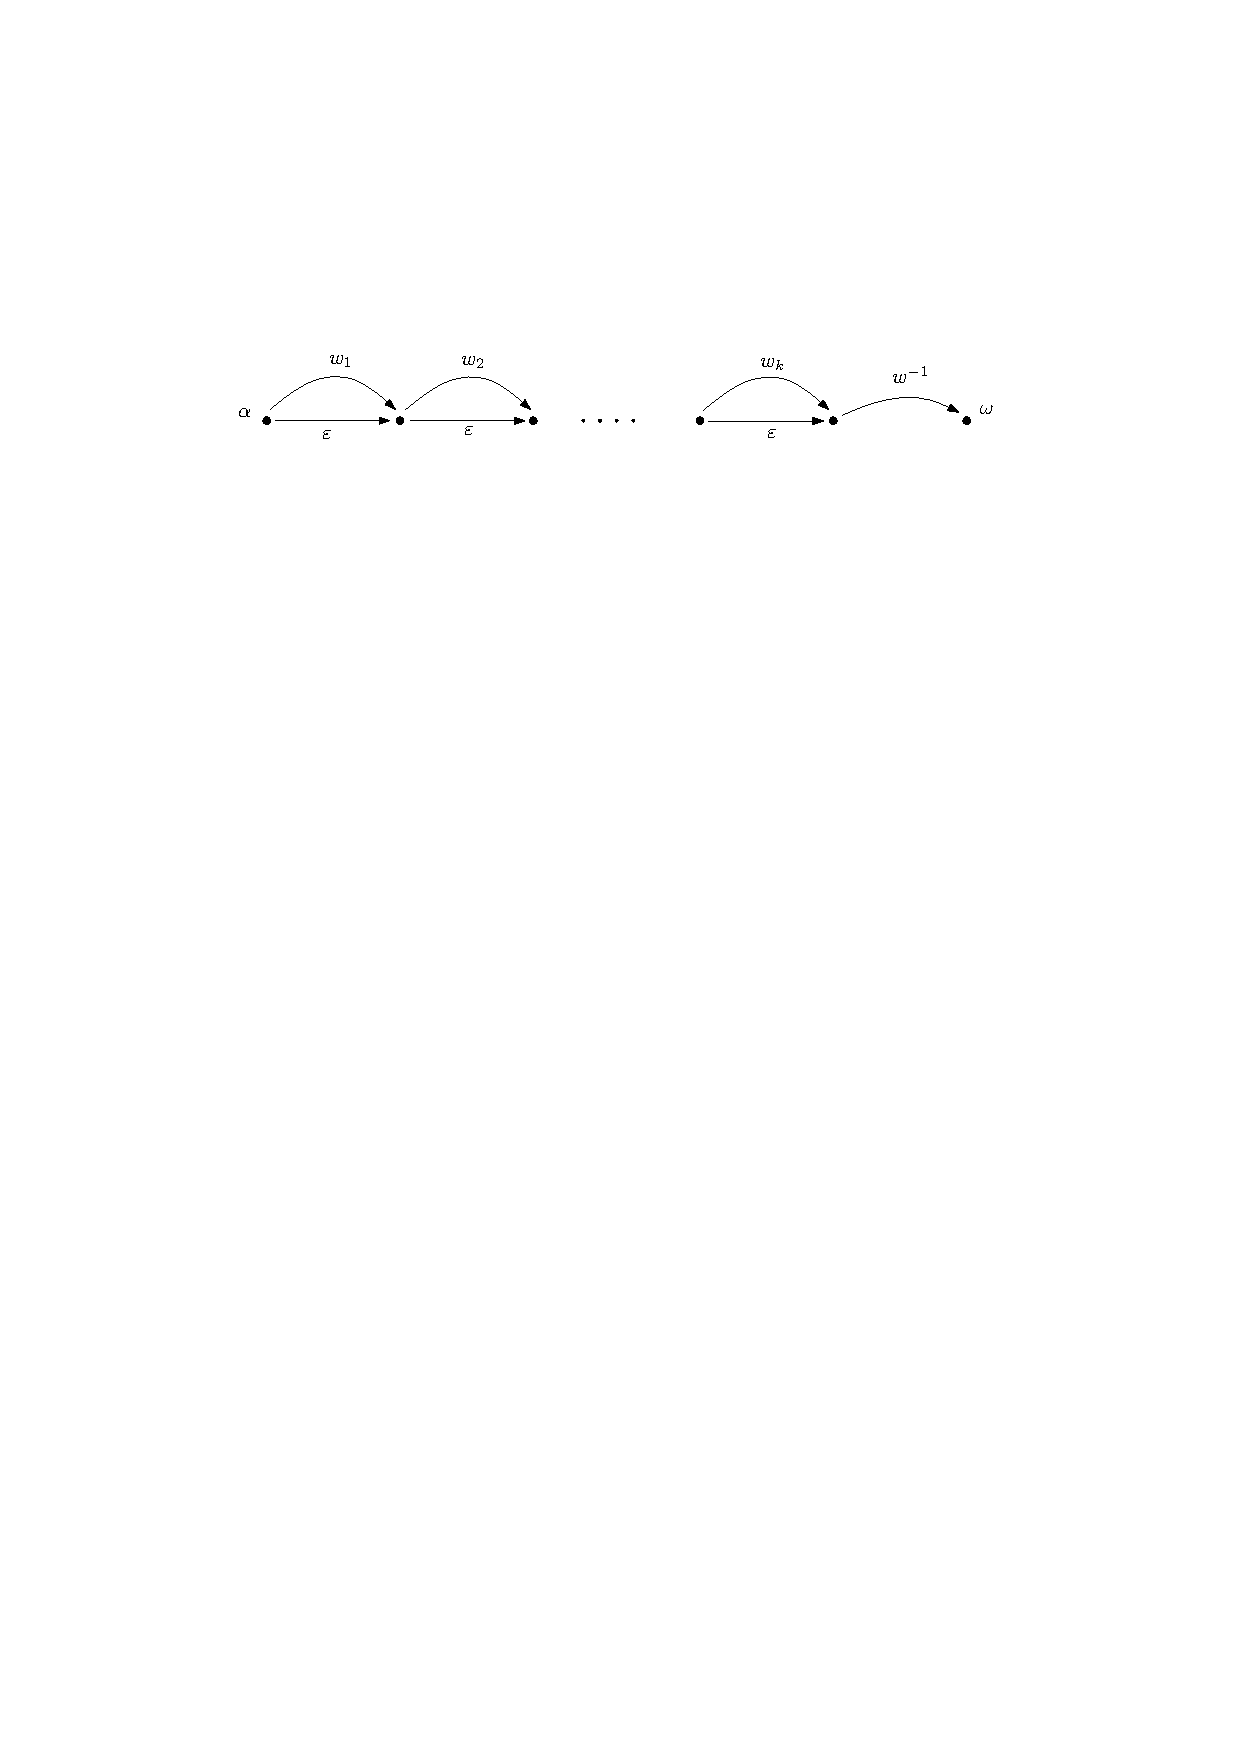
\includegraphics[width=4.5in]{ssp.pdf}
 \caption{Graph $\Gamma(w_1,w_2,\ldots,w_k,w)$, Proposition~\ref{pr:reduction_to_agp}.}\label{fi:SSP}
\end{figure}
Since that $\BKP(G)$ $\P$-time reduces to $\SSP(G)$ (see~\cite{MNU1}), it is only left to prove that $\BSMP(G)$ reduces to $\AGP(G)$. Indeed, let $(w_1,w_2,\ldots,w_k,w,1^n)$ be an input of $\BSMP(G)$. Consider the graph $\Delta=\Delta(w_1,w_2,\ldots,w_k,w,1^n)$ shown in the Fig.~\ref{fi:BSMP}.
\begin{figure}[h]
 \centering
 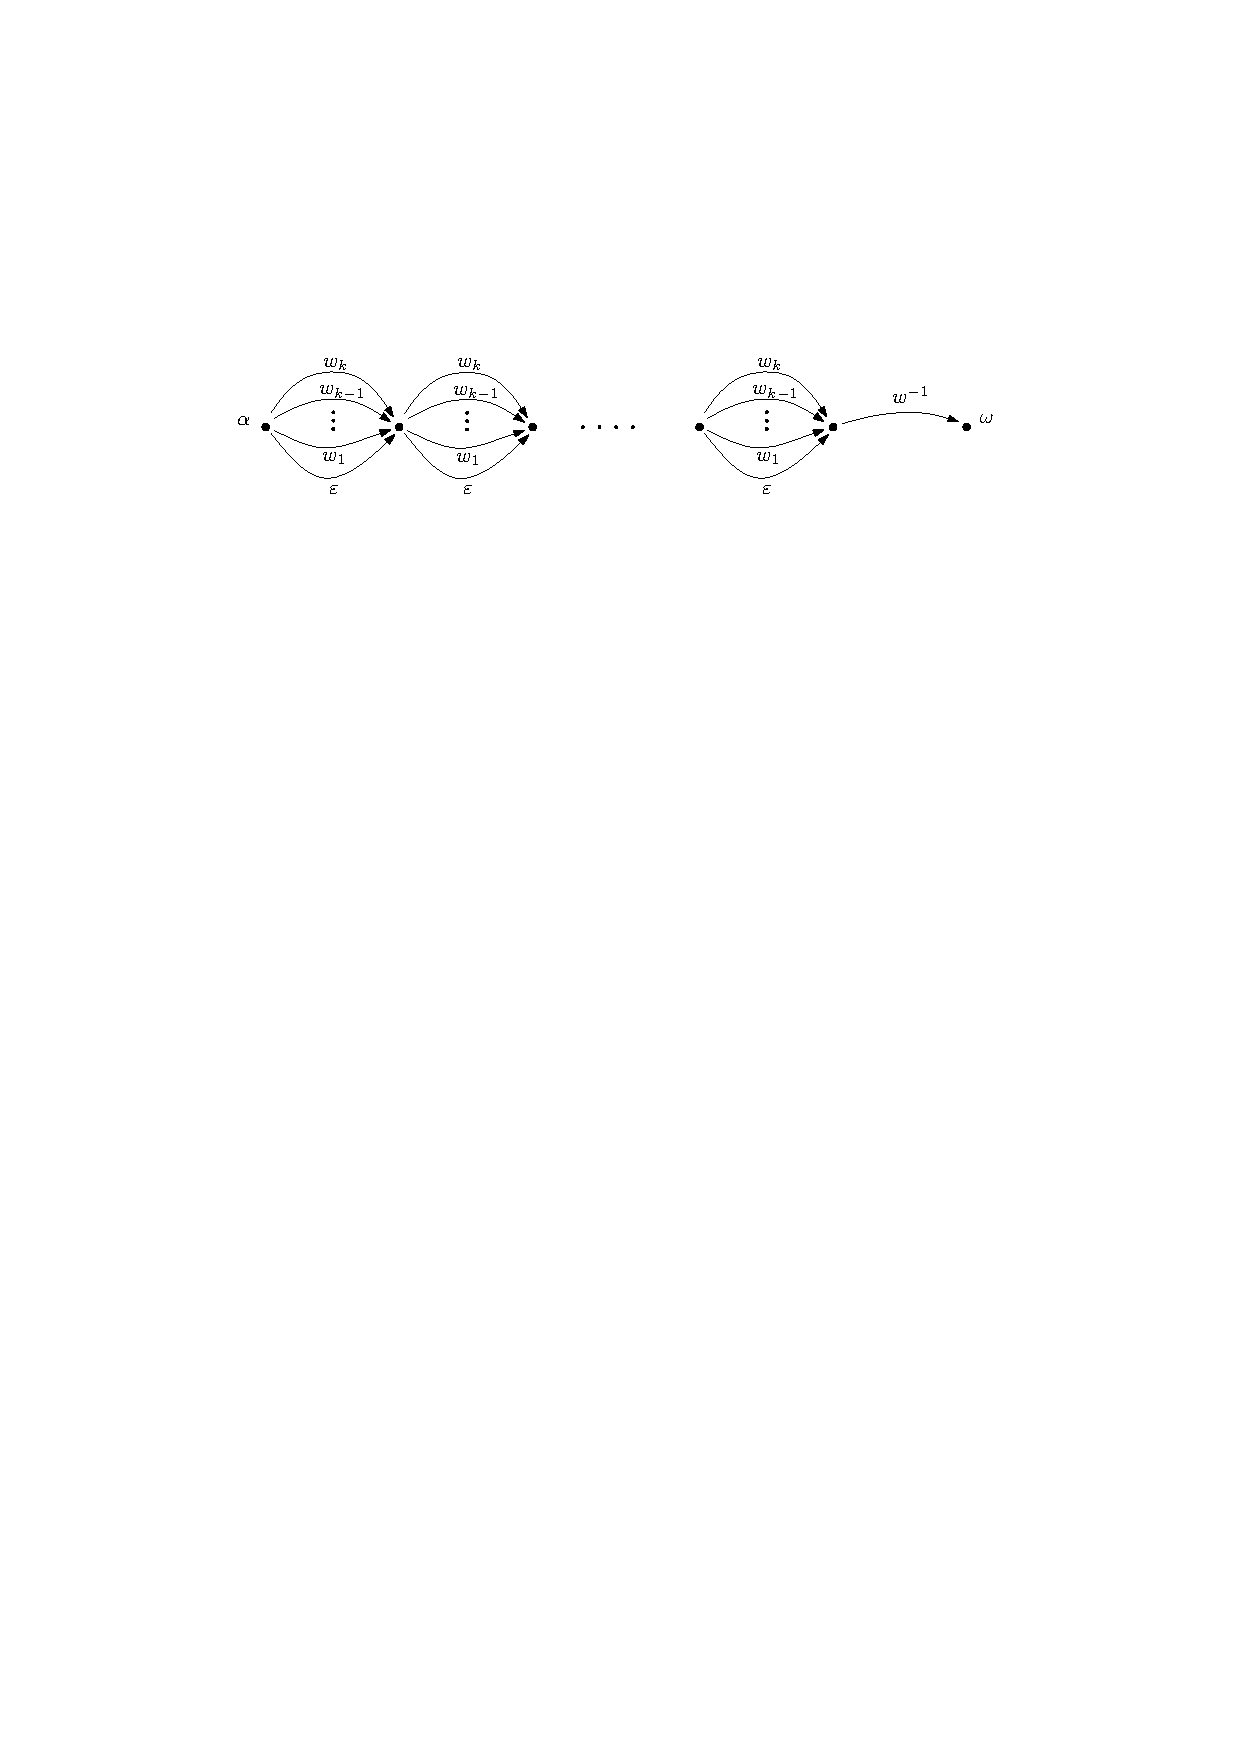
\includegraphics[width=4.5in]{bsmp.pdf}
 \caption{Graph $\Delta(w_1,w_2,\ldots,w_k,w,1^n)$, Proposition~\ref{pr:reduction_to_agp}. There are $n+2$ vertices in the graph.}\label{fi:BSMP}
\end{figure}
\end{proof}

While it still remains to be seen whether $\AGP$ reduces to either of the problems in Proposition~\ref{pr:reduction_to_agp}, in every case when it is known that those problems are $\P$-time, so is $\AGP$.
\begin{proposition}\label{pr:agp_nilp}
$\AGP(G)\in\P$ for every finitely generated virtually nilpotent group $G$.
\end{proposition}
\begin{proof}
Follows immediately from polynomial growth of virtually nilpotent functions~\cite{Wolf}, similar to the proof Theorem~3.3 in~\cite{MNU1}.
\end{proof}

\begin{proposition}\label{pr:agp_hyp}
$\AGP(G)\in\P$ for every finitely generated hyperbolic group $G$.
\end{proposition}
\begin{proof}
The statement follows immediately from~\cite[Proposition 5.5]{MNU1}.
\end{proof}

Now note that while we show in the next section that free product preserves polynomial time $\AGP$, the direct product of groups may change the complexity of $\AGP$ dramatically.
\begin{proposition}
There exist groups $G,H$ such that $\AGP(G),\AGP(H)\in\P$, but $\AGP(G\times H)$ is $\NP$-complete.
\end{proposition}
\begin{proof}
It was shown in~\cite[Theorem 7.4]{MNU1} that $\BSMP(F_2\times F_2)$ is $\NP$-complete. By Proposition~\ref{pr:reduction_to_agp} it follows that $\AGP(F_2\times F_2)$ is $\NP$-complete, while by Proposition~\ref{pr:agp_nilp} $\AGP(F_2)\in\P$.
\end{proof}

\section{$\AGP$ in free products}\label{sec:free_prod}
\begin{theorem}
If $G,H$ are groups such that $\AGP(G),\AGP(H)\in\P$ then $\AGP(G*H)\in\P$.
\end{theorem}
\begin{proof}
Let $G$ be given by a generating set $X$, and $H$ by $Y$. Let $\Gamma=\Gamma_0$ be the given acyclic graph labeled by $\Sigma=X\cup X^{-1}\cup Y\cup Y^{-1}\cup\{\varepsilon\}$. Given the graph $\Gamma_k$, $k\in\mathbb Z$, construct graph $\Gamma_{k+1}$ by adding edges to $\Gamma_k$ as follows.

Consider $\Gamma_{k}'$, the maximal subgraph of $\Gamma_k$ labeled by  $X\cup X^{-1}\cup \{\varepsilon\}$ (i.e. the graph obtained by removing all edges labeled by $Y\cup Y^{-1}$).
For each pair of vertices $v_1,v_2\in V(\Gamma_k)$, decide whether a word equal to $1$ in $G$ is readable as a label of an oriented path in $\Gamma_k'$, using polynomial time solution to $\AGP(G,X)$.
Let $E$ be the set of pairs $(v_1,v_2)\in V(\Gamma_k)\times V(\Gamma_k)$ such that the answer to the above question is positive, and there is no edge $v_1\overset{\varepsilon}{\to}v_2$ in $\Gamma_k.$ Construct the graph $\overline{\Gamma}_k$ by adding edges  $v_1\overset{\varepsilon}{\to}v_2$, $(v_1,v_2)\in E$ to the graph $\Gamma_k$.
Now consider the maximal subgraph $\Gamma_k''$ of $\overline{\Gamma}_k$ labeled by $Y\cup Y^{-1}\cup \{\varepsilon\}$ and perform similar operation using polynomial time solution to $\AGP(H,Y)$, obtaining the graph $\overline{\overline{\Gamma}}_k=\Gamma_{k+1}$.
Note that by the construction, $\size(\Gamma_{k+1})<2\size(\Gamma)^2$.

We claim that a word $w$ equal to $1$ in $G*H$ is readable from $\alpha$ to $\omega$ in $\Gamma$ if and only if there is an edge $\alpha\overset{\varepsilon}{\to}\omega$ in the graph $\Gamma_{\size(\Gamma)}$.
Indeed, suppose there is a path in $\Gamma_k$ from $\alpha$ to $\omega$ labeled by a word $w=w_1w_2\cdots w_m$, with $w_j\in \Sigma$ and at least one nontrivial letter among $w_1,\ldots, w_m$, such that $w=1$ in $G*H$.
The normal form theorem for free products guarantees that $w$ has a subword $w'=w_iw_{i+1}\cdots w_j$ of letters in $X\cup X^{-1}\cup \{\varepsilon\}$ or $Y\cup Y^{-1}\cup \{\varepsilon\}$ with $w'=1$ in $G$ or $H$, respectively, with at least one nontrivial letter among $w_i,\ldots,w_j$.
By the construction, the word $w_1\cdots w_{i-1}\varepsilon w_{j+1}\cdots w_m$ is readable as a label of a path in $\Gamma_{k+1}$ from $\alpha$ to $\omega$. Since the graph $\Gamma$ is acyclic, $m< \size(\Gamma)$.
By induction, a word $\varepsilon^{<\size(\Gamma)}$ is readable as a label of an oriented path in $\Gamma_{\size(\Gamma)-1}$ from $\alpha$ to $\omega$.
By the construction, $\Gamma_{\size(\Gamma)}$ contains an edge $\alpha\overset{\varepsilon}{\to}\omega$.
The converse direction of the claim is evident.
%Draw $\varepsilon$-edges in the graph.
\end{proof}
\begin{corollary}
$\SSP$, $\KP$, $\BSMP$, $\AGP$ are polynomial time decidable in free products of finitely generated virtually nilpotent and hyperbolic groups in any finite amount.
\end{corollary}

\section{Knapsack problem in free products}\label{sec:knapsack}
For an element $f$ of a free product of groups $G*H$, let $\|f\|$ denote the {\em syllable length} of $f$, i.e. its geodesic length in generators $G\cup H$ of $G*H$. We say that $f$ is {\em \dumb} if $f$ can be conjugated by an element of $G*H$ into $G\cup H$, i.e.
\begin{equation}\label{eq:simple}
f=u^{-1}f'u,
\end{equation}
where $u\in G*H, \|f'\|\le 1$. Otherwise, we say that $f$ is {\em \nondumb}.

\begin{lemma}\label{le:power}
Let $G,H$ be groups and let an element $f\in G\ast H$ be \nondumb.
%, $f\notin\bigcup_{u\in G*H} G^u\cup H^u$.
Then there are $a_1,\ldots,a_r\in G\cup H$, $b_1,\ldots,b_s\in G\cup H$, $c_1,\ldots,c_t\in G\cup H$, $r+t\le 2\|f\|$, $s\le \|f\|$, such that for every integer $n\ge 3$ the normal form of $f^n$ is
$$
a_1\cdots a_r(b_1\cdots b_s)^{n-2}c_1\cdots c_t.
$$
\end{lemma}
\begin{proof} Follows from the normal form theorem for free products.
\end{proof}

The statement below is, in some sense, a strengthened big-powers condition for a free product.
\begin{proposition}\label{pr:big_power}
There exists a polynomial $p(x)$ with the following property. Let $G,H$ be groups. If for $f_1,f_2,\ldots, f_m, f\in G*H$ there exist non-negative integers $n_1,n_2,\ldots,n_m\in\mathbb Z$ such that
$$
f_1^{n_1}f_2^{n_2}\cdots f_m^{n_m}=f
$$
then there exist such integers $n_1,\ldots,n_m$ with
$$n_i\le p(\|f_1\|+\|f_2\|+\ldots+\|f_m\|+\|f\|)\mbox{ whenever } f_i\mbox{ is \nondumb}.
$$
%for each $i$ such that $f_i$ is \nondumb.
\end{proposition}
\begin{proof}
For each \nondumb\ $f_i$ pass to the form of $f_i^{n_i}$ provided by Lemma~\ref{le:power}. Then inspect the equality in the Cayley graph of $G*H$ with respect to generators $G\cup H$, use pigeonhole principle to find large mutually cancelling pieces of $f_i^{n_i}$ and some $f_j^{n_j}$.
\end{proof}

\begin{proposition}
If $G,H$ are groups such that $\KP(G),\KP(H)\in\P$, then $\KP(G*H)$ is $\P$-time reducible to $\BKP(G*H)$.
\end{proposition}
\begin{proof}
Let $f_1,f_2,\ldots,f_m,f\in G*H$ be an input of $\KP(G*H)$. For each $f_i$, we can represent $f_i^{n_i}$ by their normal forms using Lemma~\ref{le:power} or simplicity of $f_i$. Suppose some $n_1,n_2,\ldots,n_m$ provide a solution to $\KP$, i.e. $f_1^{n_1}\cdots f_m^{n_m}f^{-1}=1$ in $G*H$. Representing $f^{-1}$ and each $f_i^{n_i}$ by their normal forms and combining like terms we obtain (without loss of generality) a product
\begin{equation}\label{eq:norm_form}
g_1h_1g_2h_2\cdots g_kh_k=1,
\end{equation}
where each $g_i\in G$ and each $h_i\in H$, and $k\le \|f\|+m\cdot (\max\{\|f_i\|\})\cdot p(\max\{\|f_i\|\})$ by Proposition~\ref{pr:big_power}, so $k\le N^2p(N)$ where $N$ is the total length of the input. Further, since the product in~\eqref{eq:norm_form} represents the trivial element, it can be reduced to $1$ by a series of eliminations of trivial syllables and combining like terms:
\begin{align*}
g_1h_1g_2h_2\cdots g_kh_k&=\\
g_1^{(1)}h_1^{(1)}\cdots g_k^{(1)}h_k^{(1)}&=\\
g_1^{(2)}h_1^{(2)}\cdots g_{k-1}^{(2)}h_{k-1}^{(2)}&=\\
\ldots=g_1^{(k)}h_1^{(k)}&=1,\\
\end{align*}
where the product labeled by $(j)$ is obtained from the one labeled by $(j-1)$ by a single elimination of a trivial term and combining the two (cyclically) neighboring terms. Observe that each $g_i^{(j)}$ is (up to a cyclic shift) a product of the form $g_\alpha g_{\alpha+1}\cdots g_\beta$; similarly for $h_i^{(j)}$. Therefore, each $g_i^{(j)}$ is of the form
\begin{equation}\label{eq:g_ij}
g_i^{(j)}=a_1^{\delta_1} a_2^{\delta_2}\cdots a_{k_{ij}}^{\delta_{k_{ij}}},
\end{equation}
where each $a_\mu$, $1\le \mu\le k_{ij}$ is either
\begin{itemize}
\item[(NS)] one of the syllables involved in Lemma~\ref{le:power} or ``u'' part of~\eqref{eq:simple}, in which case $\delta_\mu=1$, or
\item[(S)]\label{li:simple} the syllable $f'$ in~\eqref{eq:simple} for some $f_\nu$, in which case $\delta_\mu=n_\nu$.
\end{itemize}
Finally, note that by~\eqref{eq:g_ij} for each $j$, $k_{1j}+k_{2j}+\cdots +k_{k-j+1,j}\le Nk\le N^3p(N)$.

Now, given the equality $g_i^{(j)}=1$ for some $i,j$, if the option~(S) takes place for any $1\le \mu\le k_{ij}$, then the corresponding equality can be represented as a positive instance of the $\KP(G)$ with input of length bounded by $(N k_{ij})^2\le N^6p^2(N)$. Since $\KP(G)\in\P$, it follows that every $n_\nu$ that occurs as some $\delta_\mu$ in some $g_i^{(j)}$ is bounded by a polynomial $p_G(N)$. Similar argument takes place for the $H$-syllables $h_i^{(j)}$, resulting in a polynomial bound $p_H(N)$.

It is only left to note that since for every $1\le \nu\le m$, either $f_\nu$ is non-simple and then $n_\nu$ is bounded by $p(N)$, or it is simple and then $n_\nu$ is bounded by $p_G(N)$ or $p_H(N)$, so every $n_\nu$ is bounded by $p(N)+p_G(N)+p_H(N)$.
%we note that each $g_i$ has the form 
\end{proof}


%\bibliography{../../main_bibliography}
\bibliography{main_bibliography}
%\printindex

\end{document}

